\documentclass[arhiv]{../izpit}
\usepackage{fouriernc}
\usepackage{xcolor}
\usepackage{tikz}
\usepackage{fancyvrb}
\usetikzlibrary{calc,shapes.multipart,chains,arrows,fit,shapes}
\VerbatimFootnotes{}


\begin{document}
	
	\izpit{Programiranje I: 2. izpit}{25.\ avgust 2020}{
		Čas reševanja je 150 minut.
		Veliko uspeha!
	}
	
	%%%%%%%%%%%%%%%%%%%%%%%%%%%%%%%%%%%%%%%%%%%%%%%%%%%%%%%%%%%%%%%%%%%%%%%

	\naloga 
  
	\podnaloga Napišite funkcijo za izračun kota med dvema ravninskima vektorjema.
  \begin{verbatim}
    angle_between: float * float -> float * float -> float
  \end{verbatim}

  \podnaloga Napišite funkcijo, ki sezname dolžine tri pretvori v trojico, sicer pa vrne \verb|None|. 
  \begin{verbatim}
    list_to_triple : 'a list -> ('a * 'a * 'a) option
  \end{verbatim}

  \podnaloga Definirajte zapisni tip \verb|counter| s celoštevilskimi polji \verb|lt|, \verb|eq| in \verb|gt|. Funkcija \verb|compare_with| sprejme seznam in vrednost ter vrne koliko elementov seznama je manjših, enakih oziroma večjih kot podana vrednost. Rezultat naj bo tipa \verb|counter|, za vse točke pa naj se funkcija po seznamu sprehodi zgolj enkrat.
  \begin{verbatim}
    compare_with : 'a list -> 'a -> counter
	\end{verbatim}
	
  \podnaloga Napišite funkcijo, ki sestavi kompozitum seznama funkcij. 
  \begin{verbatim}
    apply_all : ('a -> 'a) list -> 'a -> 'a
	\end{verbatim}
  Kot primer, \verb|apply_all [f1; f2; f3]| vrne funkcijo, ki \verb|x| preslika v \verb|f1(f2(f3(x)))|. Za vse točke naj bo kompozitum sestavljen tako, da med izvajanjem ne pride do stack overflow napake. Kot test lahko uporabite:
  \begin{verbatim}
    let long_test = List.init 1000000 (fun _ -> (+) 1) in
    apply_all long_test 0
  \end{verbatim}

  \naloga
  
  Za razvrščanje točk v ravnini uporabljamo \emph{delilna drevesa}. Vozlišča drevesa razdelijo ravnino (po $x$ ali $y$ koordinati), v listih pa se nahaja seznam vseh elementov v podravnini.
  	\begin{verbatim}
    type xytree = 
      | Xsplit of int * xytree * xytree
      | Ysplit of int * xytree * xytree
      | Elements of (int * int) list
  	\end{verbatim}
  
  Vozlišče \verb|Xsplit (2, lt, rt)| ravnino razdeli glede na premico $x=2$. V poddrevesu \verb|lt| se nahajajo točke s prvo koordinato \emph{manjšo ali enako} 2, v \verb|rt| pa točke s prvo koordinato večjo od 2. Vrstni red točk v seznamih ni pomemben.
	
  \podnaloga Definirajte primer delilnega drevesa \verb|example|, ki ga prikazuje slika. Točke naj bodo vstavljene v pravilno podravnino.
	
	\[
    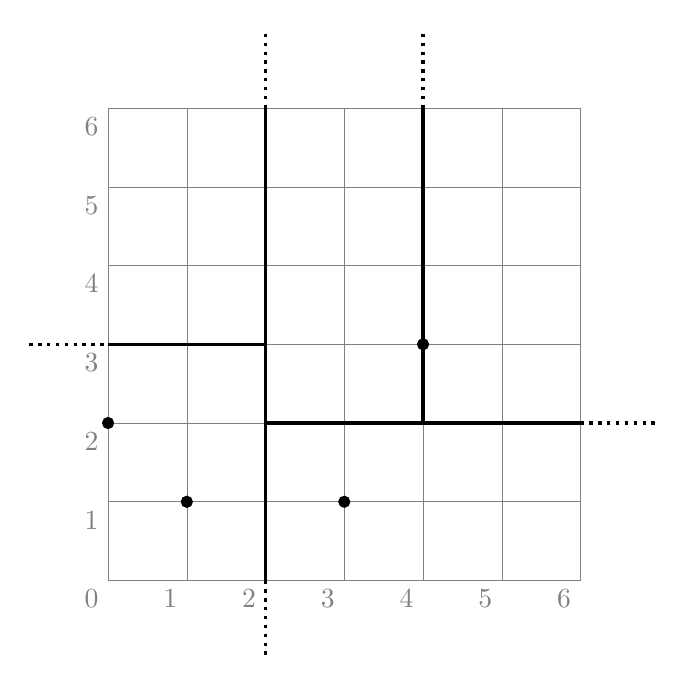
\begin{tikzpicture}

    \draw[very thick, dotted] (2,0) -- (2,-1);
    \draw[very thick, dotted] (2,6) -- (2,7);
    \draw[very thick, dotted] (-1,3) -- (0,3);
    \draw[very thick, dotted] (6,2) -- (7,2);
    \draw[very thick, dotted] (4,6) -- (4,7);

    \foreach \i in {0,...,6} {
        \draw [very thin,gray] (\i,0) -- (\i,6)  node [below left] at (\i,0) {$\i$};
    }
    \draw [very thin,gray] (0,0) -- (6,0);
    \foreach \i in {1,...,6} {
        \draw [very thin,gray] (0,\i) -- (6,\i) node [below left] at (0,\i) {$\i$};
    }
	
    \draw[very thick] (2,0) -- (2,6);
    \draw[very thick] (0,3) -- (2,3);
    \draw[very thick] (2,2) -- (6,2);
    \draw[very thick] (4,2) -- (4,6);

    \filldraw[black] (1,1) circle (2pt);
    \filldraw[black] (0,2) circle (2pt);
    \filldraw[black] (3,1) circle (2pt);
    \filldraw[black] (4,3) circle (2pt);
  \end{tikzpicture}
  \]
	
  \podnaloga Napišite funkcijo \verb|num_of_elements|, ki prešteje število točk, ki jih vsebuje delilno drevo.
  \begin{verbatim}
	# num_of_elements example;;
	- : int = 4
	\end{verbatim}
	
  \podnaloga Definirajte funkcijo \verb|insert| za vstavljanje točk v delilno drevo.
    
  \podnaloga Definirajte funkcijo \verb|alternates|, ki preveri ali delilno drevo izmenično uporablja delilno koordinato. To pomeni, da če na prvem koraku ravnino delimo glede na $x$-os, jo v drugem glede na $y$ in tako naprej.

  \podnaloga Napišite funkcijo \verb|boxed_correctly|, ki preveri ali so vsi elementi v delilnem drevesu v pravilnem vozlišču. 

  \naloga
  
  \emph{Nalogo lahko rešujete v Pythonu ali OCamlu.}

  \emph{Parnost} permutacije~$\pi$ definiramo kot parnost števila njenih \emph{inverzij}, torej takih parov števil $i < j$, da velja $\pi_i > \pi_j$. Na primer, identična permutacija je soda, ker nima inverzij, permutacija
  \[
    \rho = \begin{pmatrix}1 & 2 & 3 & 4 \\ 2 & 3 & 4 & 1 \end{pmatrix}
  \]
  pa je liha, saj ima tri inverzije: $\rho_1 > \rho_4$, $\rho_2 > \rho_4$ in $\rho_3 > \rho_4$. Enostavno lahko preverimo (pa tudi pri \emph{Algebri 1} ste se učili), da:
  \begin{itemize}
    \item je kompozitum dveh sodih ali dveh lihih permutacij soda permutacija,
    \item je kompozitum sode in lihe permutacije liha permutacija,
    \item je cikel $(1 2 3 \dots n)$ liha permutacija natanko tedaj, kadar je $n$ sod.
  \end{itemize}

  Napišite funkcijo \verb|soda|, ki sprejme naravno število $n$ in ob vsakem klicu vrne naključno izbrano \emph{sodo} permutacijo prvih $n$ naravnih števil. Funkcija naj deluje v času $O(n)$, porabi naj največ $O(n)$ dodatnega prostora, vsaka permutacija pa naj se pojavi z enako verjetnostjo (ki je za $n < 2$ enaka $1$, sicer pa $\frac{2}{n!}$). Pravilnost rešitve utemeljite v komentarjih.

\end{document}